\section{运动学里的反问题}\label{sec:01.11}

以上各节讨论的问题,都是当已知运动的轨迹函数$\vec{r}\left(t\right)$后,
求速度和加速度。在运动学中还会遇到一种相反的问题:已知质
点在各时刻的速度$\vec{v}\left(t\right)$,求它的轨迹函数$\vec{r}\left(t\right)$;已知加速度$\vec{a}\left(t\right)$,
求它的$\vec{v}\left(t\right)$。以前各节讨论的问题多与微分运算相联系,而这些
反问题,却是与积分运算相联系的。

仍然先讨论直线运动。如果已知直线运动的质点的速度为
$v\left(t\right)$,并已知在$t=0$时,质点在$x\left(0\right)$(称为初始位置),求在时刻
t的质点的坐标$x\left(t\right)$。

我们把零到$t$这段时间间隔,分成许多小段,即$\Delta t_1 , \Delta t_2 , \cdots$,
而且$\Delta t_1+\Delta t_2+\cdots=t$,如果所有各小段都相当小,则在每个间隔
中速度变化不太大,在$\Delta t_i$中速度近似为$v\left(t_i\right)$。这样,在每个时
间间隔中质点的坐标变化分别近似为:
\begin{equation*}
  \begin{array}{l}
    \Delta x_{1} \approx v\left(t_{1}\right) \Delta t_{1} \\[-1pt]
    \Delta x_{2} \approx v\left(t_{2}\right) \Delta t_{2} \\[-1pt]
    \cdots \cdots
  \end{array}
\end{equation*}
因而,质点在0到$t$间隔中坐标的总变化$x\left(t\right)-x\left(0\right)$就应当等于
这许多小变化的总和,即\vspace{-0.5em}
\begin{equation}\label{eqn:01.11.01}
  \begin{aligned}
    x\left(t\right)-x\left(0\right) & =\Delta x_{1}+\Delta x_{2}+\Delta x_{3}+\cdots    \\[-1pt]
                                    & \approx \sum_{i} v\left(t_{i}\right) \Delta t_{i}
  \end{aligned}
\end{equation}
各时间间隔$\Delta t_i$取得越小,计算结果就越准确,当所有$\Delta t_i\rightarrow 0$时,
就得到质点位置变化的精确值:

~\vspace{-1.56em}
\begin{equation}\label{eqn:01.11.02}
  x\left(t\right)=x\left(0\right)+\lim _{\Delta t_{i} \rightarrow 0} \sum_{i} v\left(t_{i}\right) \Delta t_{i}
\end{equation}
上式取极限的项,与积分的定义是一样的。所以它可写成
\begin{equation}\label{eqn:01.11.03}
  x\left(t\right)=x\left(0\right)+\int_{0}^{t} v\left(t\right) {~\mathrm d} t
\end{equation}
这就是我们所要求的答案。

现在说明式\eqref{eqn:01.11.01}或\eqref{eqn:01.11.02}中求和运算的几何意义。我
们在图\ref{fig:01.24}中画出了速度$v$对时间$t$的关系曲线。各时间间隔$\Delta t_1 , \Delta t_2 , \cdots$,相应于横坐标上的各小段,各$v\left(t_1\right) , v\left(t_2\right) , \cdots$,相应
于各小段中$ v $的近似值。因而$\Delta x_1 , \Delta x_2 , \cdots$,在数值上就等于相
应的小长方形的面积。故对所有$\Delta x_i$求和,在各小段$\Delta x_i$都趋于
无限小的情况下,在数值上就等于零到$t$间横轴之上与曲线$v$之
下所围的面积。

利用这种几何性质,对一些简单情况,计算式\eqref{eqn:01.11.03}中的
积分是很容易的。下面举两个例子。

\begin{figure}[!h]
  \begin{minipage}[b]{14em}
    \centering
    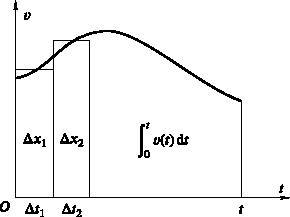
\includegraphics[width=0.8\linewidth]{figure/fig01.24}
    \caption{运动的$v-t$图}
    \label{fig:01.24}
  \end{minipage}\hfill
  \begin{minipage}[b]{14em}
    \centering
    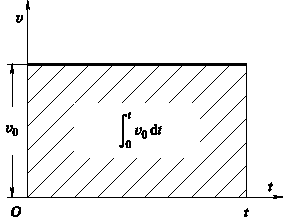
\includegraphics[width=0.8\linewidth]{figure/fig01.25}
    \caption{匀速运动的$v-t$图}
    \label{fig:01.25}
  \end{minipage}
\end{figure}

\setcounter{example}{0}
\example 匀速运动。

如果质点的速度是常数$v_0$,它的$v-t$图就如图\ref{fig:01.25}所示。由0
到$t$的横轴与曲线$v$围成一个长方形,它的面积是$v_0t$,将之代入
式\eqref{eqn:01.11.03},即得轨迹函数为:
\begin{equation}\label{eqn:01.11.04}
  x\left(t\right)=x\left(0\right)+v_0 t
\end{equation}
~\vspace{-1.5em}
\begin{figure}[!h]
  \begin{minipage}[b]{14em}
    \centering
    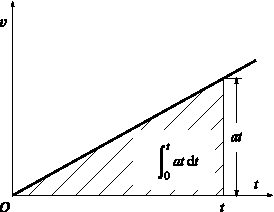
\includegraphics[width=0.8\linewidth]{figure/fig01.26}
    \caption{匀加速运动的$v \mathdash t$图}
    \label{fig:01.26}
  \end{minipage}\hfill
  \begin{minipage}[b]{14em}
    \centering
    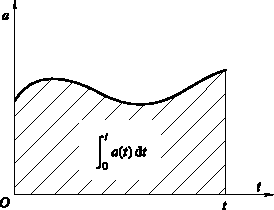
\includegraphics[width=0.8\linewidth]{figure/fig01.27}
    \caption{运动的$a-t$图}
    \label{fig:01.27}
  \end{minipage}
\end{figure}

\example 匀加速运动。

设质点的速度与时间成正比,$v=at$,在图\ref{fig:01.26}中画出这个
关系。零到$t$的横轴与曲线$v$围成一个直角三角形,它的面积是
$\dfrac{1}{2} a t^2$,代入式\eqref{eqn:01.11.03},就得到轨迹函数为:
\begin{equation*}\label{eqn:01.11.04i}
  x\left(t\right)=x\left(0\right)+\frac{1}{2}at^2 \tag{1.11.4$'$}
\end{equation*}

已知加速度$a\left(t\right)$,求速度$v\left(t\right)$的方法,同样可以按上面的方
法求得,将0到$t$的时间间隔分成小段$\Delta t_1 , \Delta t_2 , \cdots$,每个小段中
加速度分别近似为$a\left(t_1\right) , a\left(t_2\right) , \cdots$,因而在每个小段中,速度的
变化相应为$\Delta v_1\approx a\left(t_1\right)\Delta t_1 , \Delta v_2\approx a\left(t_2\right)\Delta t_2 , \cdots$,在0到$t$间隔中速
度总的变化等于所有变化之和,即
\begin{equation}\label{eqn:01.11.05}
  \begin{aligned}
    v\left(t\right)-v\left(0\right) & =\Delta v_{1}+\Delta v_{2}+\cdots                 \\
                                    & \approx \sum_{i} a\left(t_{i}\right) \Delta t_{i}
  \end{aligned}
\end{equation}
其中$v\left(0\right)$是$t=0$时质点的速度,称为初速度。
同样,取所有$\Delta t _ i \to 0$的极限,就得到速度变化的精确表达式为,
\begin{equation}\label{eqn:01.11.06}
  \begin{aligned}
    v\left(t\right) & =v\left(0\right)+\lim _{\Delta t_{i} \rightarrow 0} \sum_ i a\left(t_{i}\right) \Delta t_{i} \\
                    & =v\left(0\right)+\int_{0}^{t} a\left(t\right) {~\mathrm d} t
  \end{aligned}
\end{equation}
上式中积分的几何意义是$a-t$图中由0到$t$的横轴与$a$曲线之间
所围的面积(图\ref{fig:01.27})。

对于曲线运动的情况,式\eqref{eqn:01.11.03}、\eqref{eqn:01.11.06}分别推广成
{\setlength{\mathindent}{4em}
%\setlength\abovedisplayskip{0pt}
%\setlength\belowdisplayskip{0pt}
%\setlength{\lineskip}{-1pt}
%\setlength{\lineskiplimit}{-1pt}
\begin{eqnarray}
  \label{eqn:01.11.07}
  \begin{aligned}
    \vec{r}\left(t\right)= & \vec{r}\left(0\right)+\int_{0}^{t} \vec{v}\left(t\right) {~\mathrm d} t \\
    =                      & \vec{r}\left(0\right)
    +\left(\int_{0}^{t} v_{x}\left(t\right) {~\mathrm d} t\right) \vec{i}
    +\left(\int_{0}^{t} v_{y}\left(t\right) {~\mathrm d} t\right) \vec{j}                            \\
                           & +\left(\int_{0}^{t} v_{z}\left(t\right) {~\mathrm d} t\right) \vec{k}
  \end{aligned} \\
  \label{eqn:01.11.08}
  \begin{aligned}
    \vec{v}\left(t\right)= & \vec{v}\left(0\right)+\int_{0}^{t} \vec{a}\left(t\right) {~\mathrm d} t \\
    =                      & \vec{v}\left(0\right)
    +\left(\int_{0}^{t} a_{x}\left(t\right) {~\mathrm d} t\right) \vec{i}
    +\left(\int_{0}^{t} a_{y}\left(t\right) {~\mathrm d} t\right) \vec{j}                            \\
                           & +\left(\int_{0}^{t} a_{z}\left(t\right) {~\mathrm d} t\right) \vec{k}
  \end{aligned}
\end{eqnarray}
\setlength{\mathindent}{6em}}%
其中$\vec{r}\left(0\right)$及$\vec{v}\left(0\right)$分别为初始时刻质点的位置矢量及速度矢量。具
体使用式\eqref{eqn:01.11.07}及\eqref{eqn:01.11.08}时,可以把它们分解成分量的关系
来计算。式\eqref{eqn:01.11.07}等价于下列三式。
{%\setlength\abovedisplayskip{0pt}
%\setlength\belowdisplayskip{0pt}
%\setlength{\lineskip}{-1pt}
%\setlength{\lineskiplimit}{-1pt}
\begin{equation}
  \begin{aligned}\label{eqn:01.11.09}
    x\left(t\right)=x\left(0\right)+\int_{0}^{t} v_{x}\left(t\right) {~\mathrm d} t \\
    y\left(t\right)=y\left(0\right)+\int_{0}^{t} v_{y}\left(t\right) {~\mathrm d} t \\
    z\left(t\right)=z\left(0\right)+\int_{0}^{t} v_{z}\left(t\right) {~\mathrm d} t
  \end{aligned}
\end{equation}}%
而式\eqref{eqn:01.11.08}等价于下列三式。
{%\setlength\abovedisplayskip{0pt}
%\setlength\belowdisplayskip{0pt}
%\setlength{\lineskip}{-1pt}
%\setlength{\lineskiplimit}{-1pt}
\begin{equation}\label{eqn:01.11.10}
  \begin{aligned}
    v_x\left(t\right)=v_x\left(0\right)+\int_{0}^{t} a_{x}\left(t\right) {~\mathrm d} t \\
    v_y\left(t\right)=v_y\left(0\right)+\int_{0}^{t} a_{y}\left(t\right) {~\mathrm d} t \\
    v_z\left(t\right)=v_z\left(0\right)+\int_{0}^{t} a_{z}\left(t\right) {~\mathrm d} t
  \end{aligned}
\end{equation}}%
这些积分中没有出现矢量,就可以按一一般方法计算,譬如上述的
面积方法就是一种可行的方法.

研究运动有两种次序。一种是先研究轨迹,已知轨迹函数为
$\vec{r}\left(t\right)$,再来推求速度$\vec{v}\left(t\right)$,加速度$\vec{a}\left(t\right)$。就人类的认识过程来说,的
确是先看到轨迹的形状,然后有了运动快慢的概念,最后认识到
速度的变化,即加速度。另一种次序是:先知道加速度,然后再
求速度及轨迹。在物理学中,从力学的规律来看。往往是如此。

前一种次序,看上去非常自然,是人类研究机械运动所走的
一条路。在牛顿之前,亚里士多德认为轨迹是最基本的,速度则
次之。这种方法的特点是先研究运动的大的整体方面,然后再涉
及局部细节。

后一种次序,是牛顿创建的方法。也是现代物理学一个基本
的方法。牛顿认为,不要先探讨物体运动的整体方面。而是先研
究运动的瞬时情况,瞬时情况更为基本。弄清瞬时情况之后再来
讨论整体运动。也可以说,这种方法是先研究局部细节,然后再
作积分,得到整体性质。至今在大多数情况下,物理学家仍采取
牛顿的这种方法。

上述两种方法反映了两种不同的信念。一种认为整体的大的
方面更简单些,因此,主张从大到小的研究顺序;另一种认为局
部的单元过程更简单些,因此。主张从小到大的研究顺序。我们
将在第五章说明,这两种“简单性”可能是分不开的。
